\begin{algebraUE}{183}
\begin{enumerate}
  \item Sei $R$ ein Unterring mit $1$ eines Körpers $K$. Dann ist
  \begin{align*}
    K^{\prime} := \left\{\frac{p}{q}: p,q \in R, q \neq 0 \right\}
  \end{align*}
  ein Unterkörper von $K$.
  \item Der Körper $K^{\prime}$ aus dem ersten Teil ist der kleinster Unterkörper
  von $K$, der $R$ enthält, symbolisch $K^{\prime} = \langle R \rangle_{\text{Körper}}$.
  Explizit bedeutet das: Jeder Unterkörper $K^{\primeprime}$ von $K$ mit $R \subseteq K^{\primeprime}$
  umfasst $K^{\prime}$.
  \item In derselben Situation ist $K$ (zusammen mit der Inklusionsabbildung) genau
  dann ein Quotientenkörper von $R$, wenn $K = K^{\prime}$ gilt.
  \item Ist $\iota: R \rightarrow K$ eine isomorphe Einbettung des Integritätsbereichs $R$
  in einen Körper $K$ und $Q$ der von $\iota(R)$ erzeugte Unterkörper von $K$,
  so ist $Q$ zusammen mit $\iota$ ein Quotientenkörper von $R$.
\end{enumerate}
\end{algebraUE}
\begin{solution}
\leavevmode \\
\begin{enumerate}
  \item Da der Körper $K$ kommutativ ist, ist auch $K^{\prime}$ bereits kommutativ.
  Mit den Rechenregeln
  \begin{align*}
    \frac{p_1}{q_1} + \frac{p_2}{q_2} = \frac{p_1q_2 + p_2q_1}{q_1q_2} \\
    \frac{p_1}{q_1}   \frac{p_2}{q_2} = \frac{p_1p_2}{q_1q_2}
  \end{align*}
  sieht man auch die Abgeschlossenheit bezüglich der Addition, sowie Multiplikation.
  Das Distributivgesetz in $K^{\prime}$ folgt ebenso aus dem Distributivgesetz in $K$ selbst.
  Damit bleiben nur noch die Nullteilerfreiheit, sowie die Existenz der multiplikativen Inversen zu überprüfen.
  Seien also $\frac{p_1}{q_1}, \frac{p_2}{q_2} \in K^{\prime}$ mit $\frac{p_1}{q_1}   \frac{p_2}{q_2} = 0$ beliebig.
  Dann gilt
  \begin{align*}
    0 = \frac{p_1}{q_1}   \frac{p_2}{q_2} = \frac{p_1p_2}{q_1q_2} \implies p_1p_2 = 0
  \end{align*}
  und aufgrund der Nullteilerfreiheit in $K:$
  \begin{align*}
    p_1 = 0 \lor p_2 = 0 \implies \frac{p_1}{q_1} = 0 \lor \frac{p_2}{q_2} = 0.
  \end{align*}
  Nun zur Existenz multiplikativer Inversen: Sei $\frac{p}{q} \in \K^{\prime}: p \neq 0$ beliebig.
  Dann ist $\frac{q}{p} \in \K^{\prime}$ und es gilt
  \begin{align*}
    \frac{p}{q}\frac{q}{p} = \frac{pq}{qp} = 1.
  \end{align*}
  Damit ist $K^{\prime}$ ein Unterkörper von $K$.
  \item Sei $K^{\primeprime}$ nun ein beliebiger Körper, welcher $R$ enthält.
  Damit muss vorerst $K^{\primeprime} \subseteq R$ gelten. Aufgrund der Abgeschlossenheit
  unter der multiplikativen Inversenbildung muss auch gelten
  \begin{align*}
    K^{\primeprime} \supseteq \left\{\frac{1}{q}: q \neq 0 \in R\right\} \cup \left\{\frac{p}{1}: p \in R\right\}
  \end{align*}
  Aufgrund der Abgeschlossenheit bezüglich der Multiplikation gilt schließlich auch
  \begin{align*}
    K^{\primeprime} \supseteq  \left\{\frac{p}{q}: q \neq 0 \in R\right\} = K^{\prime}.
  \end{align*}
  \item Gelte zuerst $K = K^{\prime}$. \\
  Da $R$ kommutativ ist, ist $R\backslash\{0\}$ ein kürzbares Untermonoid von $R$.
  Aufgrund $\frac{p}{q} := [(p,q)]_{\sim}$ mit $(p_1,q_1) \sim (p_2,q_2) :\iff p_1q_2 = p_2q_1$
  ist $K = R \times R\backslash\{0\}$ laut Satz 3.3.5.8. ein Quotientenkörper von $R$.
  Sei $K$ umgekehrt ein Quotientenkörper von $R$. Da Quotientenkörper bis auf
  Isomorphie eindeutig bestimmt sind, gilt damit  $K \cong K^{\prime}$. Es gibt also
  genau eine isomorphe Einbettung $\iota: K \rightarrow K^{\prime}$. Die Identität
  auf $K$ ist so eine Abbildung und damit folgt $K = K^{\prime}$.
  \item In Punkt 1 und 2 haben wir mit $K^{\prime}$ den kleinsten Unterkörper von $K$,
  welcher einen beliebigen Ring $R$ mit eins enthält bestimmt. Als homomorphes Bild eines
  Integritätsbereichs ist $\iota(R)$ ein Ring mit eins und wir können $Q$ angeben als
  \begin{align*}
    Q = \left\{ \frac{p}{q}: p,q \in \iota(R)\right\}.
  \end{align*}
  Aus Punkt 3 folgt schließlich, dass $Q$ ein Quotientenkörper von $\iota(R)$ ist
  und da $R$ isomorph zu $\iota(R)$ ist, auch ein Quotientenkörper von $R$.
  Um das einzusehen, betrachte einen beliebigen Körper $\widetilde{Q}$ in den $R$
  mittels $\widetilde{\iota}$ isomorph eingebettet ist:
  \begin{center}
  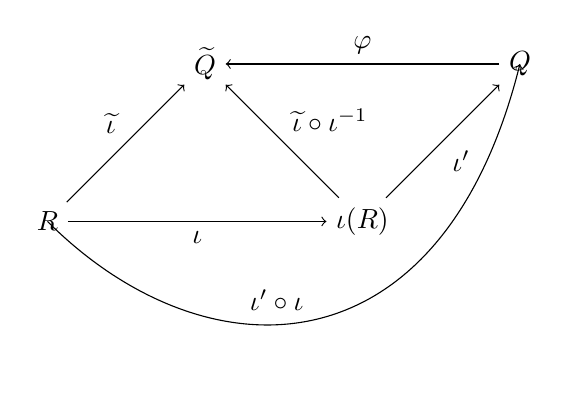
\begin{tikzpicture}[auto]
      \node (R) at (0,0) {$R$};
      \node (iotaR) at (4,0) {$\iota(R)$};
      \node (Q) at (6,2) {$Q$};
      \node (Qschlange) at (2,2) {$\widetilde{Q}$};
      \draw[->] (R) to node [swap] {$\iota$} (iotaR);
      \draw[->] (iotaR) to node [swap]  {$\iota^{\prime}$} (Q);
      \draw[->] (R) to node {$\widetilde{\iota}$} (Qschlange);
      \draw[->] (Q) to node [swap] {$\varphi$} (Qschlange);
      \draw[->] (iotaR) to node [swap] {$\widetilde{\iota}\circ\iota^{-1}$} (Qschlange);
      \draw[->] (0,0) .. controls  (2,-2) and (5,-2) .. node {$\iota^{\prime}\circ\iota$} (6,2) ;
  \end{tikzpicture} \\
  \end{center}
\end{enumerate}

\end{solution}
